\documentclass[aspectratio=169, 10pt]{beamer}

% Packages
\usepackage{graphicx}
\usepackage{booktabs}
\usepackage{tikz}
\usetikzlibrary{positioning,shapes,arrows.meta,patterns,calc,decorations.pathreplacing}
\usepackage{amsmath,amssymb}
\usepackage{algorithm}
\usepackage{algpseudocode}

% Brand colors
\definecolor{Garnet}{HTML}{73000A}
\definecolor{GarnetDark}{HTML}{500007}
\definecolor{Rose}{HTML}{CC2E40}
\definecolor{Atlantic}{HTML}{466A9F}
\definecolor{Congaree}{HTML}{1F414D}
\definecolor{Horseshoe}{HTML}{65780B}
\definecolor{Black90}{HTML}{363636}
\definecolor{Black70}{HTML}{5C5C5C}
\definecolor{Black30}{HTML}{C7C7C7}
\definecolor{Black10}{HTML}{ECECEC}

% Theme configuration - NO rounded edges
\usetheme{default}
\usecolortheme[named=Garnet]{structure}
\setbeamertemplate{navigation symbols}{}
\setbeamertemplate{blocks}[default]
\setbeamertemplate{itemize items}[square]
\setbeamertemplate{enumerate items}[square]

% Frame title formatting - sharp Garnet box
\setbeamercolor{frametitle}{fg=white, bg=Garnet}
\setbeamerfont{frametitle}{size=\Large, series=\bfseries}
\setbeamertemplate{frametitle}{
  \nointerlineskip
  \begin{beamercolorbox}[wd=\paperwidth, ht=1.2cm, dp=0.3cm]{frametitle}
    \hspace{0.5cm}\insertframetitle
  \end{beamercolorbox}
}

% Footer
\setbeamertemplate{footline}{
  \leavevmode%
  \hbox{%
  \begin{beamercolorbox}[wd=.333333\paperwidth,ht=2.5ex,dp=1ex,left]{author in head/foot}%
    \hspace{0.5cm}\footnotesize AIAA Region II Student Conference 2026
  \end{beamercolorbox}%
  \begin{beamercolorbox}[wd=.333333\paperwidth,ht=2.5ex,dp=1ex,center]{title in head/foot}%
    \footnotesize University of South Carolina
  \end{beamercolorbox}%
  \begin{beamercolorbox}[wd=.333333\paperwidth,ht=2.5ex,dp=1ex,right]{date in head/foot}%
    \footnotesize\insertframenumber{}/\inserttotalframenumber\hspace{0.5cm}
  \end{beamercolorbox}}%
  \vskip0pt%
}

% Section dividers
\AtBeginSection[]{
  \begin{frame}[noframenumbering,plain]
  \vfill
  \centering
  \begin{beamercolorbox}[sep=8pt,center,wd=\paperwidth,ht=\paperheight]{title}
    \usebeamerfont{title}\textcolor{white}{\insertsectionhead}\par
  \end{beamercolorbox}
  \vfill
  \end{frame}
}
\setbeamercolor{section page}{bg=Garnet}

% Title slide
\title{\Large\textbf{Surface-Object Detection and Tracking from Commercial X-Band Radar Using Adaptive ST-DBSCAN}}
\author{S. Cancilla, J.C. Vaught, D. Cahl, Y. Wang}
\institute{University of South Carolina, Columbia, SC 29208}
\date{AIAA Region II Student Conference 2026}

\graphicspath{{Cancilla_ST-DBSCAN/}}

\begin{document}

% Title slide with full Garnet background
{
\setbeamercolor{background canvas}{bg=Garnet}
\begin{frame}[plain,noframenumbering]
\vfill
\centering
{\Huge\textcolor{white}{\textbf{Surface-Object Detection and Tracking}}}\\[0.3cm]
{\Huge\textcolor{white}{\textbf{from Commercial X-Band Radar}}}\\[0.3cm]
{\Huge\textcolor{white}{\textbf{Using Adaptive ST-DBSCAN}}}\\[1cm]
{\large\textcolor{white}{S. Cancilla, J.C. Vaught, D. Cahl, Y. Wang}}\\[0.3cm]
{\large\textcolor{white}{University of South Carolina}}\\[0.2cm]
{\large\textcolor{white}{Columbia, SC 29208}}\\[1cm]
{\normalsize\textcolor{white}{AIAA Region II Student Conference 2026}}
\vfill
\end{frame}
}

%=============================================================================
\begin{frame}{Motivation}
\small
\vspace{-0.4cm}
\begin{columns}[T]
\column{0.5\textwidth}
\textbf{Commercial X-Band Radar Challenges:}
\begin{itemize}
  \setlength{\itemsep}{0pt}
  \setlength{\topsep}{0pt}
  \setlength{\parskip}{0pt}
  \item \textcolor{Rose}{No Doppler phase} (intensity only)
  \item Non-stationary sea clutter
  \item Heavy-tailed amplitude statistics
  \item Range-varying point density ($R^{-4}$)
  \item Intermittent target visibility
\end{itemize}

\textbf{DBSCAN Limitations:}
\begin{itemize}
  \setlength{\itemsep}{0pt}
  \setlength{\topsep}{0pt}
  \setlength{\parskip}{0pt}
  \item Fixed $\varepsilon$ fails with heterogeneous density
  \item Track fragmentation from dropouts
  \item No temporal linkage
\end{itemize}

\column{0.5\textwidth}
\vspace{-0.4cm}
\begin{figure}
  
\includegraphics[width=0.9\textwidth]{figures/sample_radar_frame.png}
  \caption{\tiny Synthetic radar frame}
\end{figure}
\end{columns}
\end{frame}

%=============================================================================
\begin{frame}{Related Work}
\scriptsize
\begin{columns}[T]
\column{0.48\textwidth}
\textbf{Classical Tracking (1960s-1980s):}
\begin{itemize}
  \item Kalman filtering (1960)
  \item MHT - Reid (1979)
  \item JPDAF - Fortmann (1983)
  \item CFAR detection - Rohling (1983)
  \item \textcolor{Rose}{Issue:} Assumes known clutter distributions
\end{itemize}

\vspace{0.3cm}
\textbf{Density-Based Clustering (1990s-2000s):}
\begin{itemize}
  \item DBSCAN - Ester et al. (1996)
  \item OPTICS - Ankerst et al. (1999)
  \item VDBSCAN - Liu et al. (2007)
  \item ST-DBSCAN - Birant \& Kut (2007)
  \item HDBSCAN - Campello et al. (2013)
\end{itemize}

\column{0.48\textwidth}
\textbf{Modern Deep Learning (2010s):}
\begin{itemize}
  \item SORT - Bewley et al. (2016)
  \item DeepSORT - Wojke et al. (2017)
  \item \textcolor{Rose}{Issue:} Require appearance features (not available in radar)
\end{itemize}

\vspace{0.3cm}
\textbf{Our Contribution:}
\begin{itemize}
  \item \textcolor{Congaree}{Adaptive $\varepsilon$ via k-NN statistics}
  \item \textcolor{Congaree}{Gap recovery for track continuity}
  \item \textcolor{Congaree}{Real-time embedded implementation}
  \item \textcolor{Congaree}{Union-Find structures for efficient merging}
\end{itemize}
\end{columns}
\end{frame}

%=============================================================================
\begin{frame}{Problem Formulation}
\scriptsize
\vspace{-0.5cm}
\begin{columns}[T]
\column{0.48\textwidth}
\textbf{Detection Set at Sweep $t$:}
\vspace{-0.15cm}
\begin{equation*}
  \mathcal{D}_t = \{ (r_i, \theta_i, I_i, t) : i = 1, \ldots, N_t \}
\end{equation*}
\vspace{-0.3cm}

\textbf{Objective:} Partition into tracks:
\vspace{-0.15cm}
\begin{equation*}
  \mathcal{D} = \mathcal{T}_1 \cup \mathcal{T}_2 \cup \cdots \cup \mathcal{T}_K \cup \mathcal{N}
\end{equation*}
\vspace{-0.3cm}

\textbf{Distance Metrics:}
\vspace{-0.15cm}
\begin{align*}
  d_s(\mathbf{p}_i, \mathbf{p}_j) &= \sqrt{(x_i - x_j)^2 + (y_i - y_j)^2} \\
  d_t(\mathbf{p}_i, \mathbf{p}_j) &= |t_i - t_j|
\end{align*}

\column{0.48\textwidth}
\vspace{-0.2cm}
\textbf{Processing Pipeline:}
\begin{center}
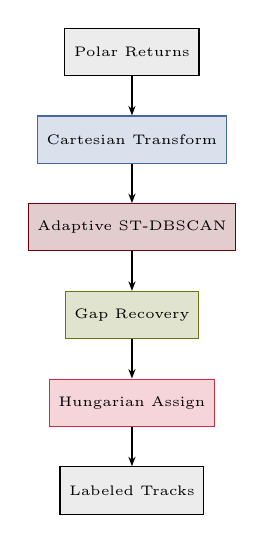
\begin{tikzpicture}[scale=0.85,
    node distance=0.5cm,
    block/.style={rectangle, draw, text=black, minimum height=0.6cm, minimum width=1.6cm, align=center, font=\tiny},
    arrow/.style={-{Stealth[length=1.2mm]}, thick}
]
\node[block, fill=Black10] (input) {Polar Returns};
\node[block, below=of input, fill=Atlantic!20, draw=Atlantic] (cart) {Cartesian Transform};
\node[block, below=of cart, fill=Garnet!20, draw=Garnet] (stdb) {Adaptive ST-DBSCAN};
\node[block, below=of stdb, fill=Horseshoe!20, draw=Horseshoe] (gap) {Gap Recovery};
\node[block, below=of gap, fill=Rose!20, draw=Rose] (hung) {Hungarian Assign};
\node[block, below=of hung, fill=Black10] (output) {Labeled Tracks};

\draw[arrow] (input) -- (cart);
\draw[arrow] (cart) -- (stdb);
\draw[arrow] (stdb) -- (gap);
\draw[arrow] (gap) -- (hung);
\draw[arrow] (hung) -- (output);
\end{tikzpicture}
\end{center}
\end{columns}
\end{frame}

%=============================================================================
\begin{frame}{Adaptive ST-DBSCAN Method}
\tiny
\vspace{-0.8cm}
\begin{columns}[T]
\column{0.48\textwidth}
\textbf{Challenge:} Fixed $\varepsilon$ fails with density variation
\vspace{-0.1cm}

\textbf{Solution:} k-NN adaptive epsilon
\vspace{-0.2cm}
\begin{equation*}
  \varepsilon_s(\mathbf{p}) = \min\left( d_k(\mathbf{p}) \cdot \alpha, \varepsilon_{s,\max} \right)
\end{equation*}
\vspace{-0.3cm}

\textbf{Global estimation:}
\vspace{-0.2cm}
\begin{equation*}
  \varepsilon_s^{\text{global}} = \text{Percentile}_{90}\left( \{ d_k(\mathbf{p}) : \mathbf{p} \in \mathcal{S} \} \right)
\end{equation*}
\vspace{-0.3cm}

\textbf{Epsilon floor:}
\vspace{-0.2cm}
\begin{equation*}
  \varepsilon_s^{\text{final}} = \max\left( \varepsilon_s^{\text{global}}, \varepsilon_{\min} \right)
\end{equation*}

\column{0.48\textwidth}
\begin{algorithm}[H]
\caption*{\textbf{Algorithm 1:} Adaptive Epsilon}
\tiny
\begin{algorithmic}[1]
\Require $\mathcal{P}$, $k$, $\beta$, $\rho$, $\varepsilon_{\min}$, $\varepsilon_{\max}$
\Ensure $\varepsilon_s$
\State $\mathcal{S} \gets$ sample $\lfloor \beta \cdot |\mathcal{P}| \rfloor$ points
\ForAll{$\mathbf{p} \in \mathcal{S}$}
    \State $d_k(\mathbf{p}) \gets$ $k$-th nearest neighbor distance
\EndFor
\State $\varepsilon_s \gets \text{Percentile}_{\rho}\left( \{ d_k(\mathbf{p}) \} \right)$
\State \Return{$\max(\varepsilon_{\min}, \min(\varepsilon_s, \varepsilon_{\max}))$}
\end{algorithmic}
\end{algorithm}
\vspace{-0.2cm}

\textbf{Parameters:} $k = 5$, $\alpha = 1.5$, $\rho = 90$, $\varepsilon_{\min} = 20$ px
\end{columns}
\end{frame}

%=============================================================================
\begin{frame}{Gap Recovery Mechanism}
\scriptsize
\begin{columns}[T]
\column{0.48\textwidth}
\textbf{Problem:} Intermittent visibility fragments tracks

\vspace{0.15cm}
\textbf{Solution:} Union-Find merging across temporal gaps

\vspace{0.15cm}
\textbf{Temporal gap:}
\begin{equation*}
  \Delta t = t_j^{\text{start}} - t_i^{\text{end}}
\end{equation*}

\textbf{Spatial gap between centroids:}
\begin{equation*}
  \Delta s = \| \bar{\mathbf{p}}_i(t_i^{\text{end}}) - \bar{\mathbf{p}}_j(t_j^{\text{start}}) \|_2
\end{equation*}

\textbf{Velocity-based threshold:}
\begin{equation*}
  d_{\max} = v_{\max} \cdot \Delta t \cdot T_s
\end{equation*}

\textbf{Merge if:} $\Delta t \leq \tau$ and $\Delta s \leq d_{\max}$

\column{0.48\textwidth}
\begin{algorithm}[H]
\caption*{\textbf{Algorithm 2:} Gap Recovery}
\scriptsize
\begin{algorithmic}[1]
\Require Clusters $\{\mathcal{T}_1, \ldots, \mathcal{T}_K\}$, $\tau$, $v_{\max}$, $T_s$
\Ensure Merged $\{\mathcal{T}'_1, \ldots, \mathcal{T}'_{K'}\}$
\State Sort clusters by $t^{\text{end}}$ ascending
\State Initialize union-find structure
\ForAll{cluster $\mathcal{T}_i$}
    \ForAll{cluster $\mathcal{T}_j$ with $t_j^{\text{start}} > t_i^{\text{end}}$}
        \State $\Delta t \gets t_j^{\text{start}} - t_i^{\text{end}}$
        \If{$\Delta t > \tau$}
            \State \textbf{break}
        \EndIf
        \State $d_{\max} \gets v_{\max} \cdot \Delta t \cdot T_s$
        \State $\Delta s \gets \| \bar{\mathbf{p}}_i - \bar{\mathbf{p}}_j \|_2$
        \If{$\Delta s \leq d_{\max}$}
            \State \Call{Union}{$\mathcal{T}_i$, $\mathcal{T}_j$}
        \EndIf
    \EndFor
\EndFor
\State \Return{clusters grouped by components}
\end{algorithmic}
\end{algorithm}
\end{columns}
\end{frame}

%=============================================================================
\begin{frame}{Hungarian Assignment}
\scriptsize
\begin{columns}[T]
\column{0.48\textwidth}
\textbf{Purpose:} Frame-to-frame track association

\vspace{0.2cm}
\textbf{Cost matrix between track centroids:}
\begin{equation*}
  C_{ij} = \| \mathbf{c}_i^{t-1} - \mathbf{d}_j^t \|_2
\end{equation*}

\vspace{0.15cm}
\textbf{Optimal assignment:}
\begin{equation*}
  \pi^* = \arg\min_{\pi} \sum_i C_{i,\pi(i)}
\end{equation*}

\vspace{0.15cm}
\textbf{Gating:} Reject assignments with $C_{ij} > \gamma$

\vspace{0.15cm}
\textbf{Benefits:}
\begin{itemize}
  \setlength{\itemsep}{0pt}
  \item Low latency for real-time output
  \item Explicit track identity maintenance
  \item Complements ST-DBSCAN clustering
\end{itemize}

\column{0.48\textwidth}
\begin{center}
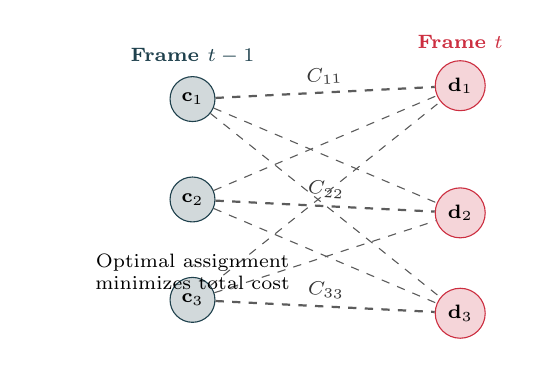
\begin{tikzpicture}[scale=0.85]
\scriptsize

% Previous frame tracks
\node[circle, draw=Congaree, fill=Congaree!20, minimum size=0.45cm] (t1) at (0,3) {$\mathbf{c}_1$};
\node[circle, draw=Congaree, fill=Congaree!20, minimum size=0.45cm] (t2) at (0,1.5) {$\mathbf{c}_2$};
\node[circle, draw=Congaree, fill=Congaree!20, minimum size=0.45cm] (t3) at (0,0) {$\mathbf{c}_3$};

% Current frame detections
\node[circle, draw=Rose, fill=Rose!20, minimum size=0.45cm] (d1) at (4,3.2) {$\mathbf{d}_1$};
\node[circle, draw=Rose, fill=Rose!20, minimum size=0.45cm] (d2) at (4,1.3) {$\mathbf{d}_2$};
\node[circle, draw=Rose, fill=Rose!20, minimum size=0.45cm] (d3) at (4,-0.2) {$\mathbf{d}_3$};

% Labels
\node[above=0.05cm of t1] {\textcolor{Congaree}{\textbf{Frame $t-1$}}};
\node[above=0.05cm of d1] {\textcolor{Rose}{\textbf{Frame $t$}}};

% Cost matrix visualization
\draw[dashed, Black70, thick] (t1) -- node[above, sloped, Black90] {$C_{11}$} (d1);
\draw[dashed, Black70] (t1) -- (d2);
\draw[dashed, Black70] (t1) -- (d3);
\draw[dashed, Black70] (t2) -- (d1);
\draw[dashed, Black70, thick] (t2) -- node[above, sloped, Black90] {$C_{22}$} (d2);
\draw[dashed, Black70] (t2) -- (d3);
\draw[dashed, Black70] (t3) -- (d1);
\draw[dashed, Black70] (t3) -- (d2);
\draw[dashed, Black70, thick] (t3) -- node[above, sloped, Black90] {$C_{33}$} (d3);

\node[below=0.3cm of t2, text width=4cm, align=center] {Optimal assignment minimizes total cost};
\end{tikzpicture}
\end{center}
\end{columns}
\end{frame}

%=============================================================================
\begin{frame}{Implementation}
\scriptsize
\begin{columns}[T]
\column{0.48\textwidth}
\textbf{Platform:} NVIDIA Jetson AGX Orin
\begin{itemize}
  \setlength{\itemsep}{0pt}
  \item Arm Cortex-A78AE (12 cores)
  \item 32 GB unified memory
  \item \textasciitilde 25 W power consumption
\end{itemize}

\vspace{0.15cm}
\textbf{Implementation:} Rust
\begin{itemize}
  \setlength{\itemsep}{0pt}
  \item Memory safety
  \item Zero-cost abstractions
  \item Predictable performance
  \item \textcolor{Congaree}{Spatial hashing} ($h = 2\varepsilon_{s,\max}$)
  \item \textcolor{Congaree}{Rayon parallelism} (k-NN queries)
  \item \textcolor{Congaree}{Union-Find} (gap recovery)
\end{itemize}

\vspace{0.15cm}
\textbf{Performance:}
\begin{itemize}
  \setlength{\itemsep}{0pt}
  \item \textcolor{Rose}{\textbf{511 $\pm$ 93 ms per sweep}}
  \item \textasciitilde 2 sweeps/s
  \item Exceeds real-time for 48 RPM radar
  \item Memory $<$ 500 MB
\end{itemize}

\column{0.48\textwidth}
\begin{table}
\centering
\scriptsize
\caption{Per-Sweep Timing Breakdown}
\begin{tabular}{@{}lc@{}}
\toprule
\textbf{Stage} & \textbf{Time (ms)} \\
\midrule
Frame loading & 7 \\
Adaptive $\varepsilon$ (k-NN) & 196 \\
ST-DBSCAN clustering & 169 \\
Cluster extraction & 34 \\
Gap recovery & 19 \\
Hungarian assignment & 3 \\
I/O (output) & 40 \\
\midrule
\textbf{Total} & \textbf{511} \\
\bottomrule
\end{tabular}
\end{table}

\vspace{0.15cm}
\textbf{Bottlenecks:}
\begin{itemize}
  \setlength{\itemsep}{0pt}
  \item k-NN computation (38\%)
  \item ST-DBSCAN clustering (33\%)
  \item Both parallelized with Rayon
\end{itemize}
\end{columns}
\end{frame}

%=============================================================================
\begin{frame}{Clustering Comparison}
\begin{figure}
\centering
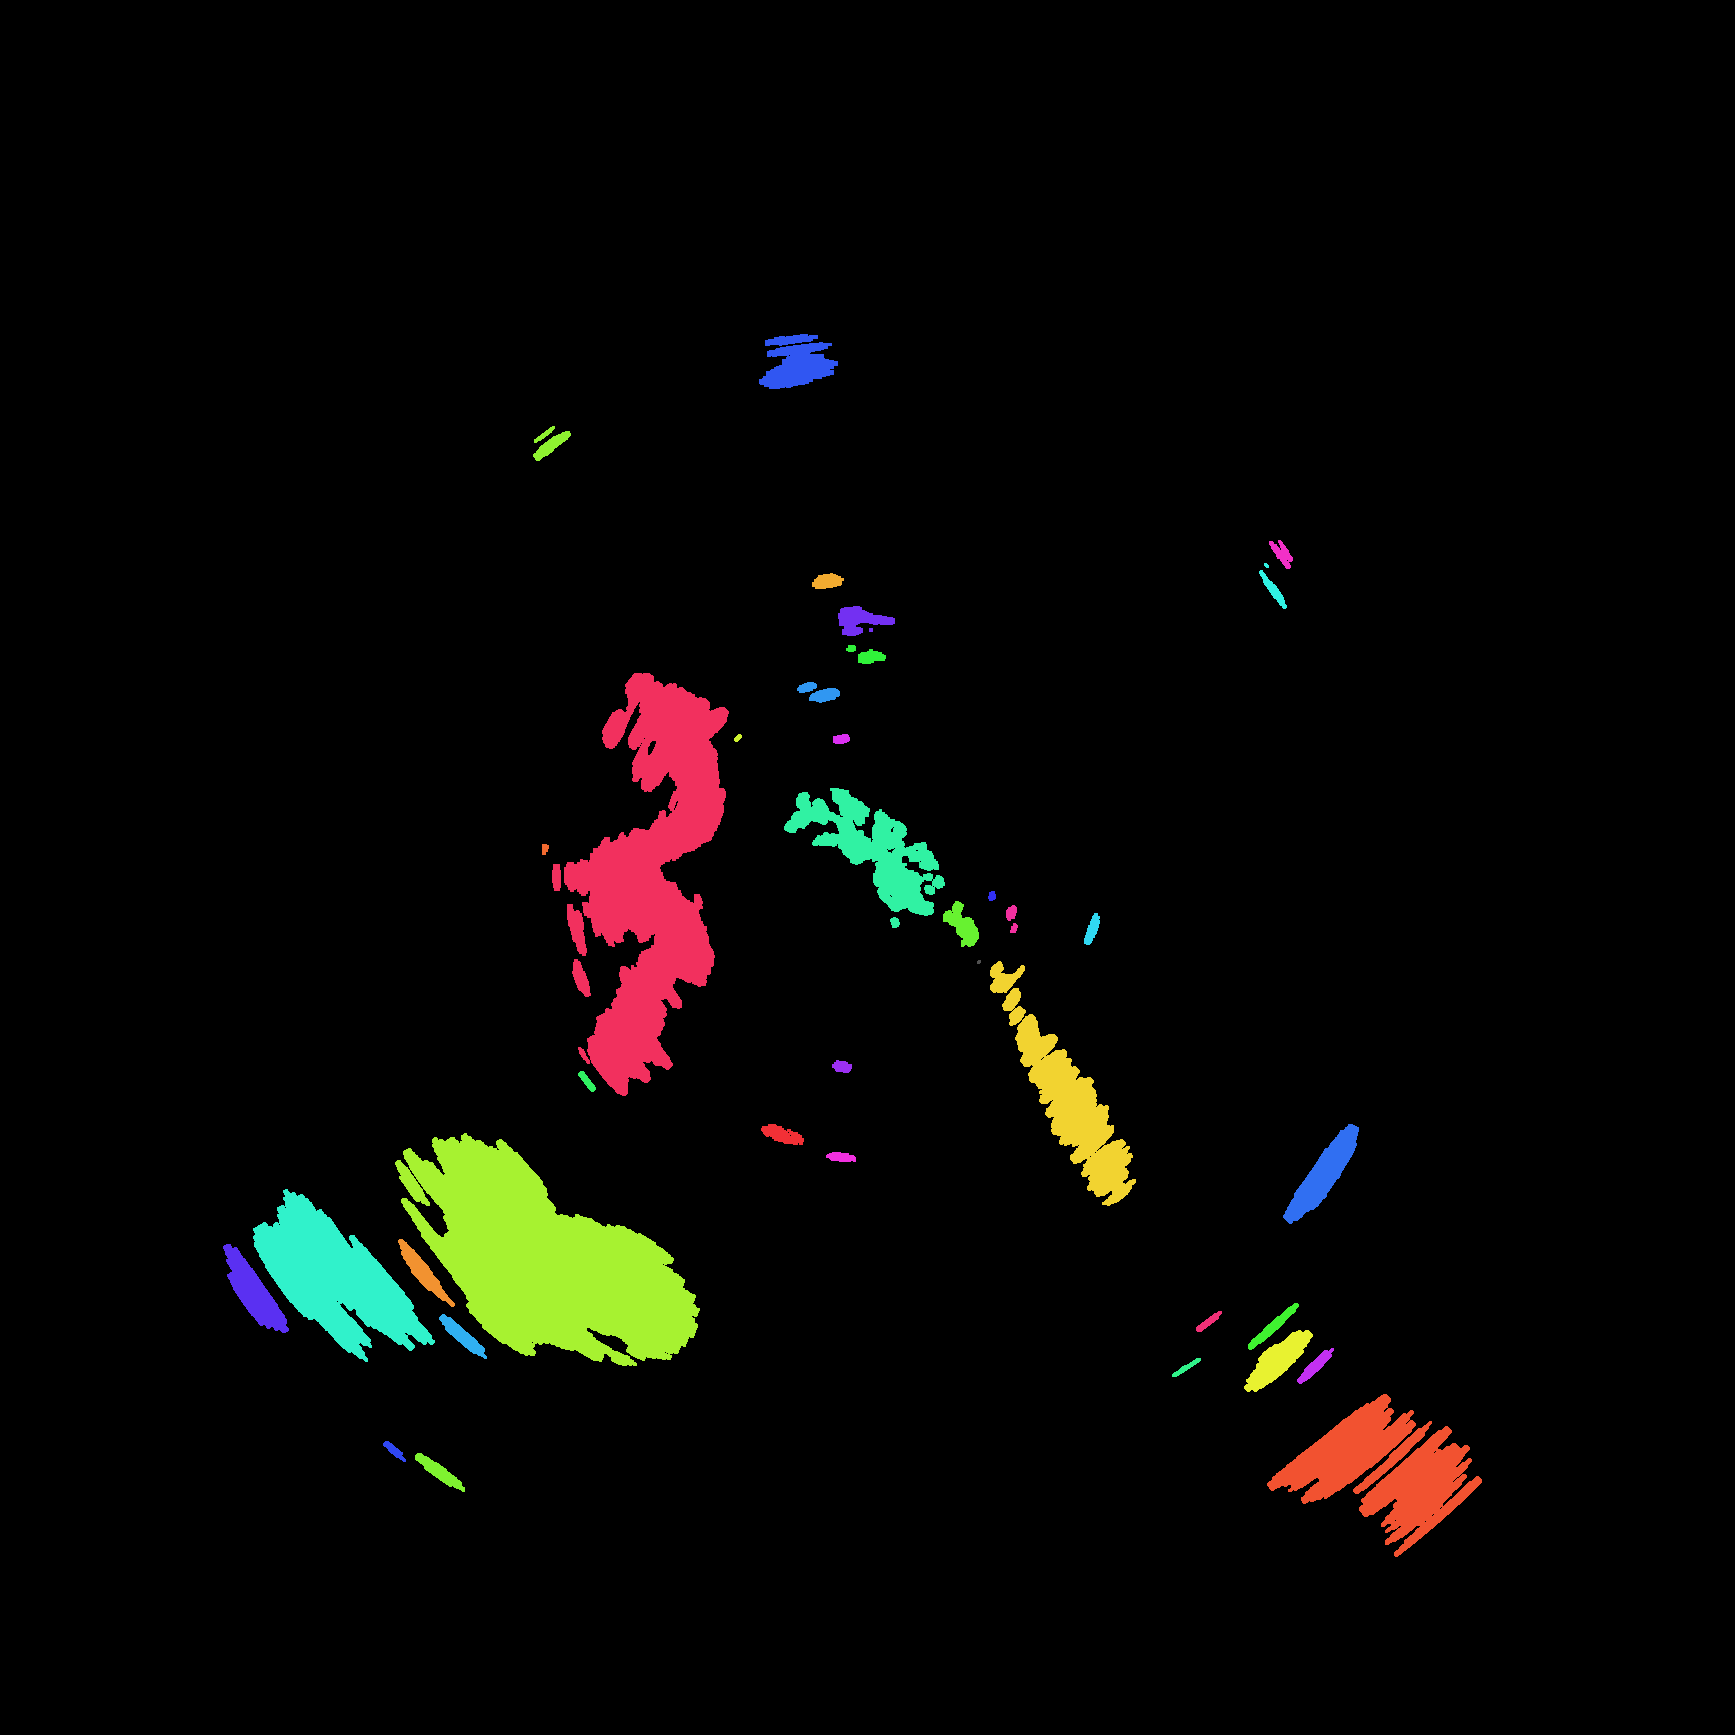
\includegraphics[width=0.31\textwidth]{figures/dbscan_frame.png}
\hfill
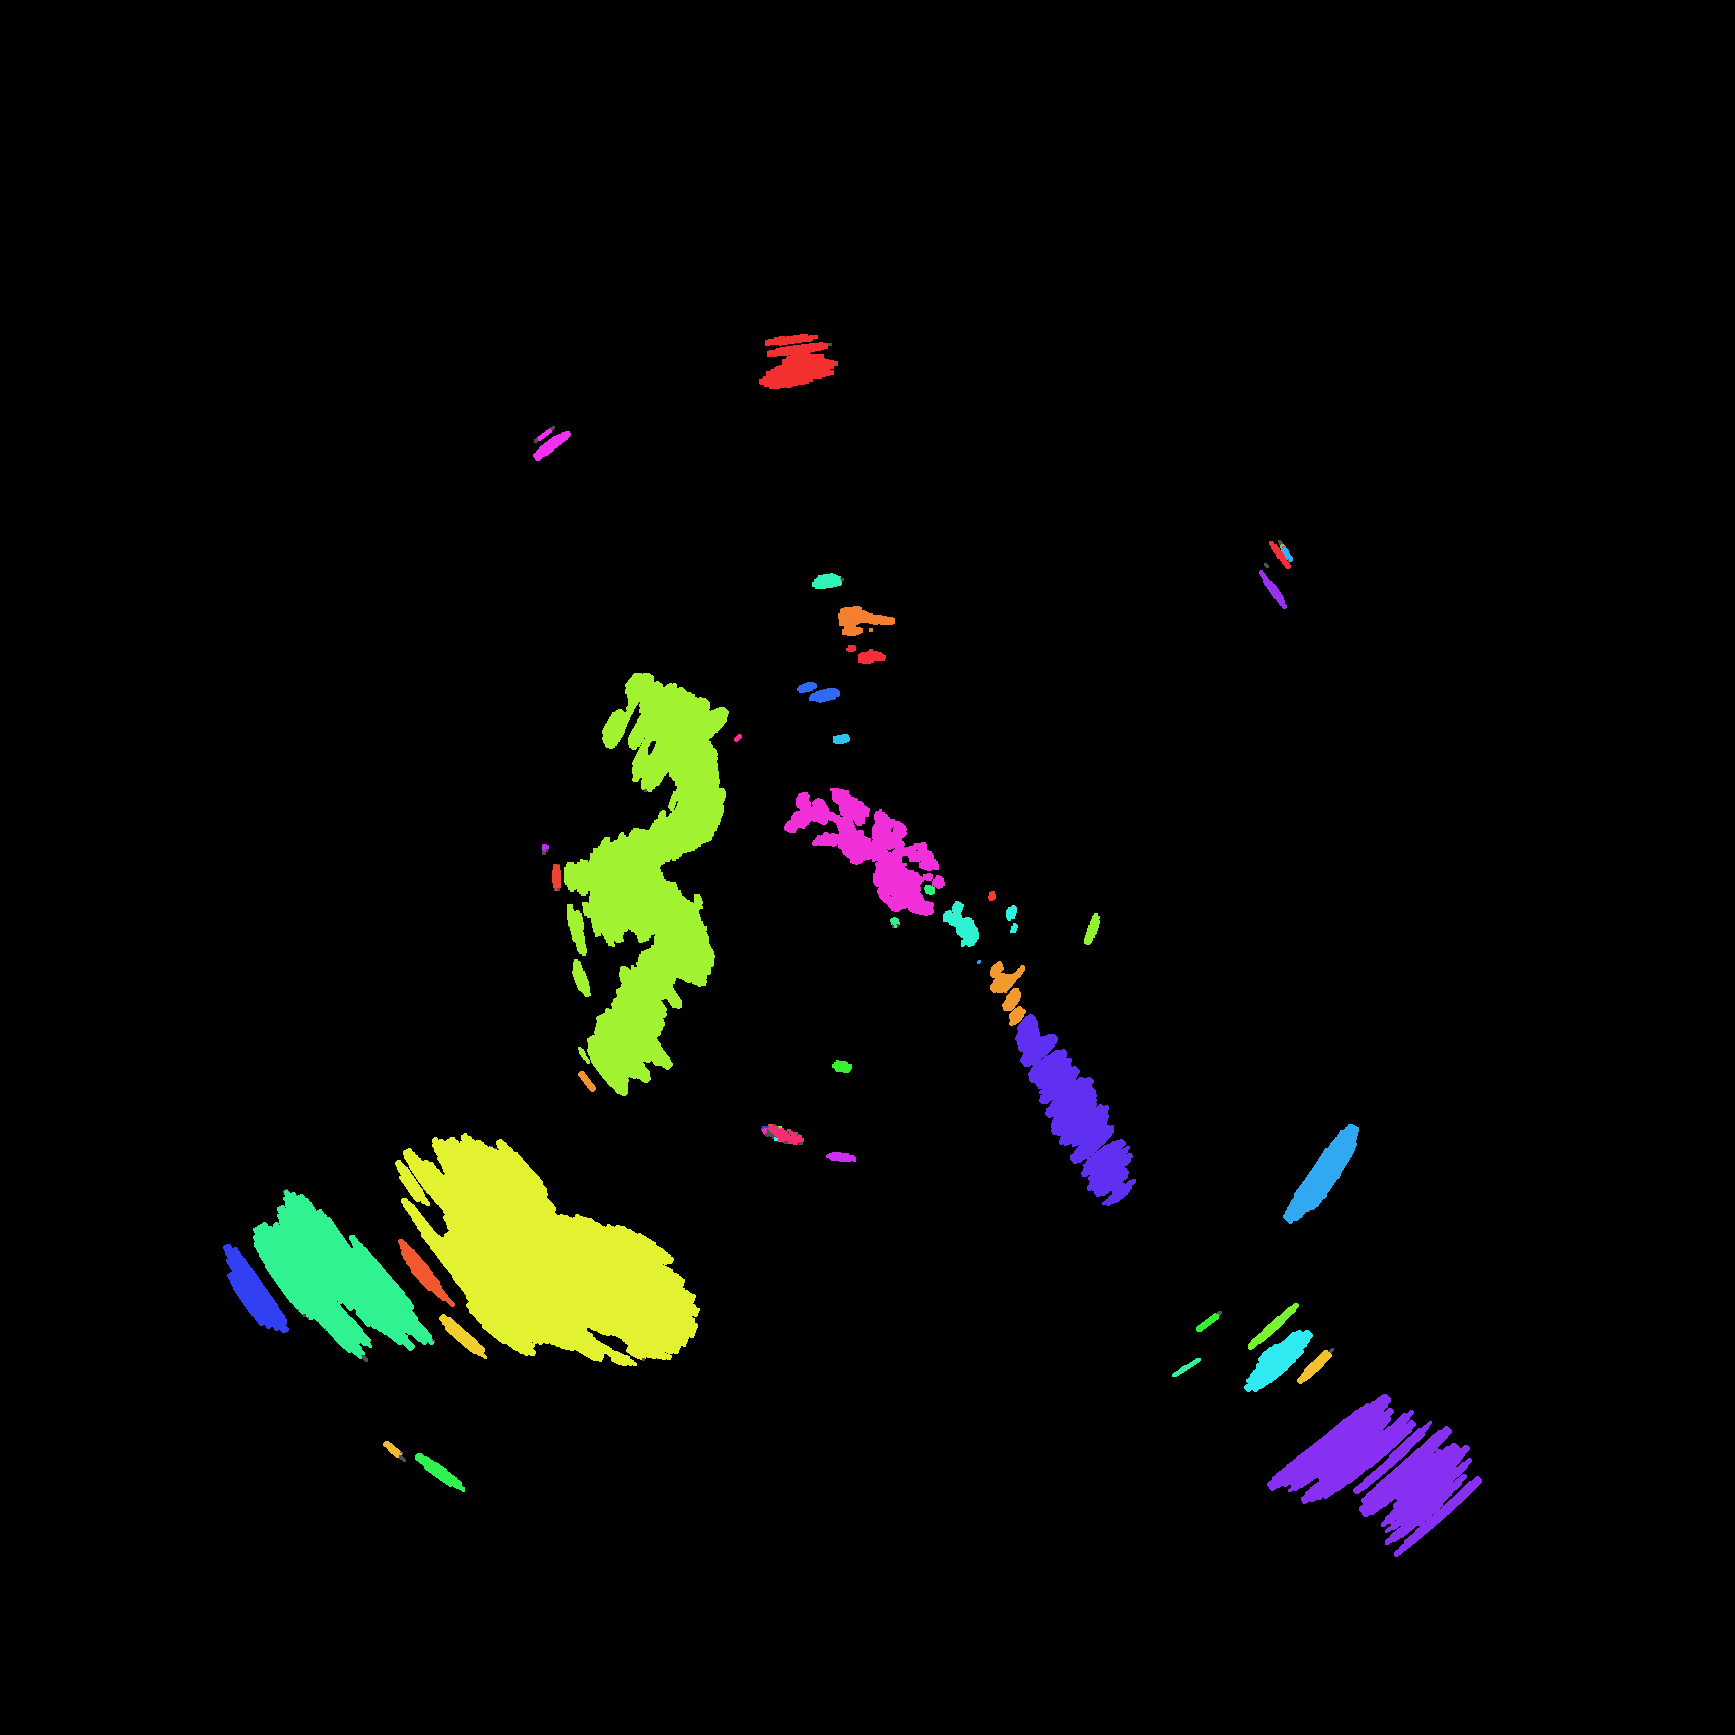
\includegraphics[width=0.31\textwidth]{figures/stdbscan_frame.png}
\hfill
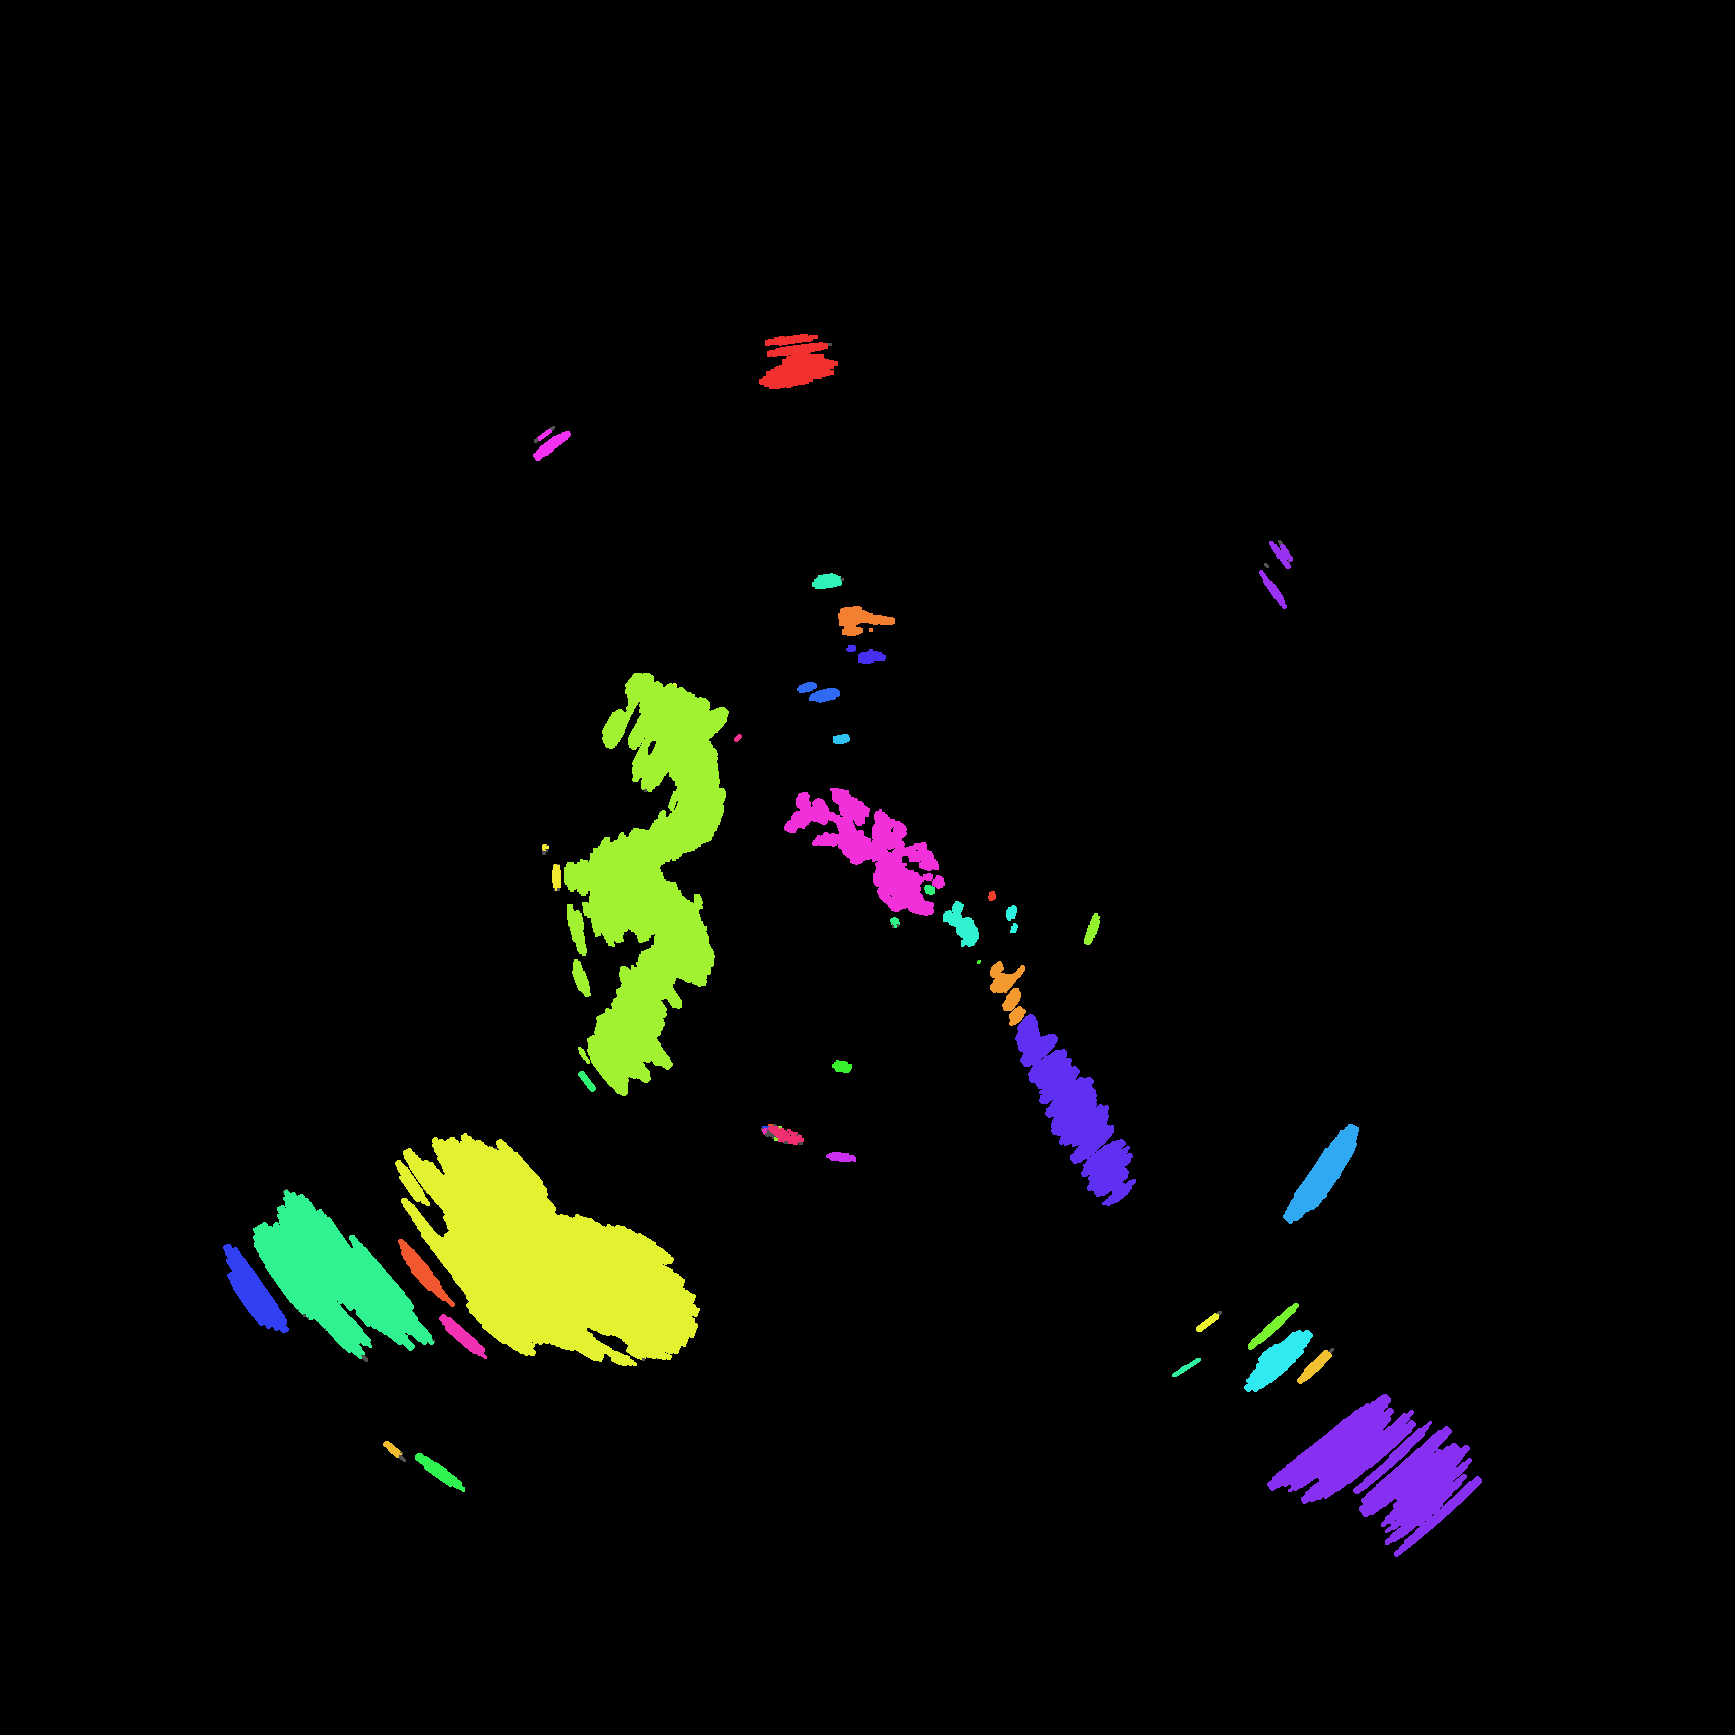
\includegraphics[width=0.31\textwidth]{figures/gap_frame.png}
\caption*{\scriptsize\textbf{Left:} Vanilla DBSCAN ($\varepsilon_s = 10$): 1693 clusters, many spurious detections. \textbf{Center:} Adaptive ST-DBSCAN ($\varepsilon_{\min} = 20$): 1177 clusters, larger spatial neighborhoods. \textbf{Right:} Adaptive + Gap Recovery: merged temporally adjacent clusters.}
\end{figure}
\end{frame}

%=============================================================================
\begin{frame}{Tracking Comparison}
\begin{figure}
\centering

\includegraphics[width=0.31\textwidth]{figures/dbscan_track_frame.png}
\hfill

\includegraphics[width=0.31\textwidth]{figures/stdbscan_track_frame.png}
\hfill
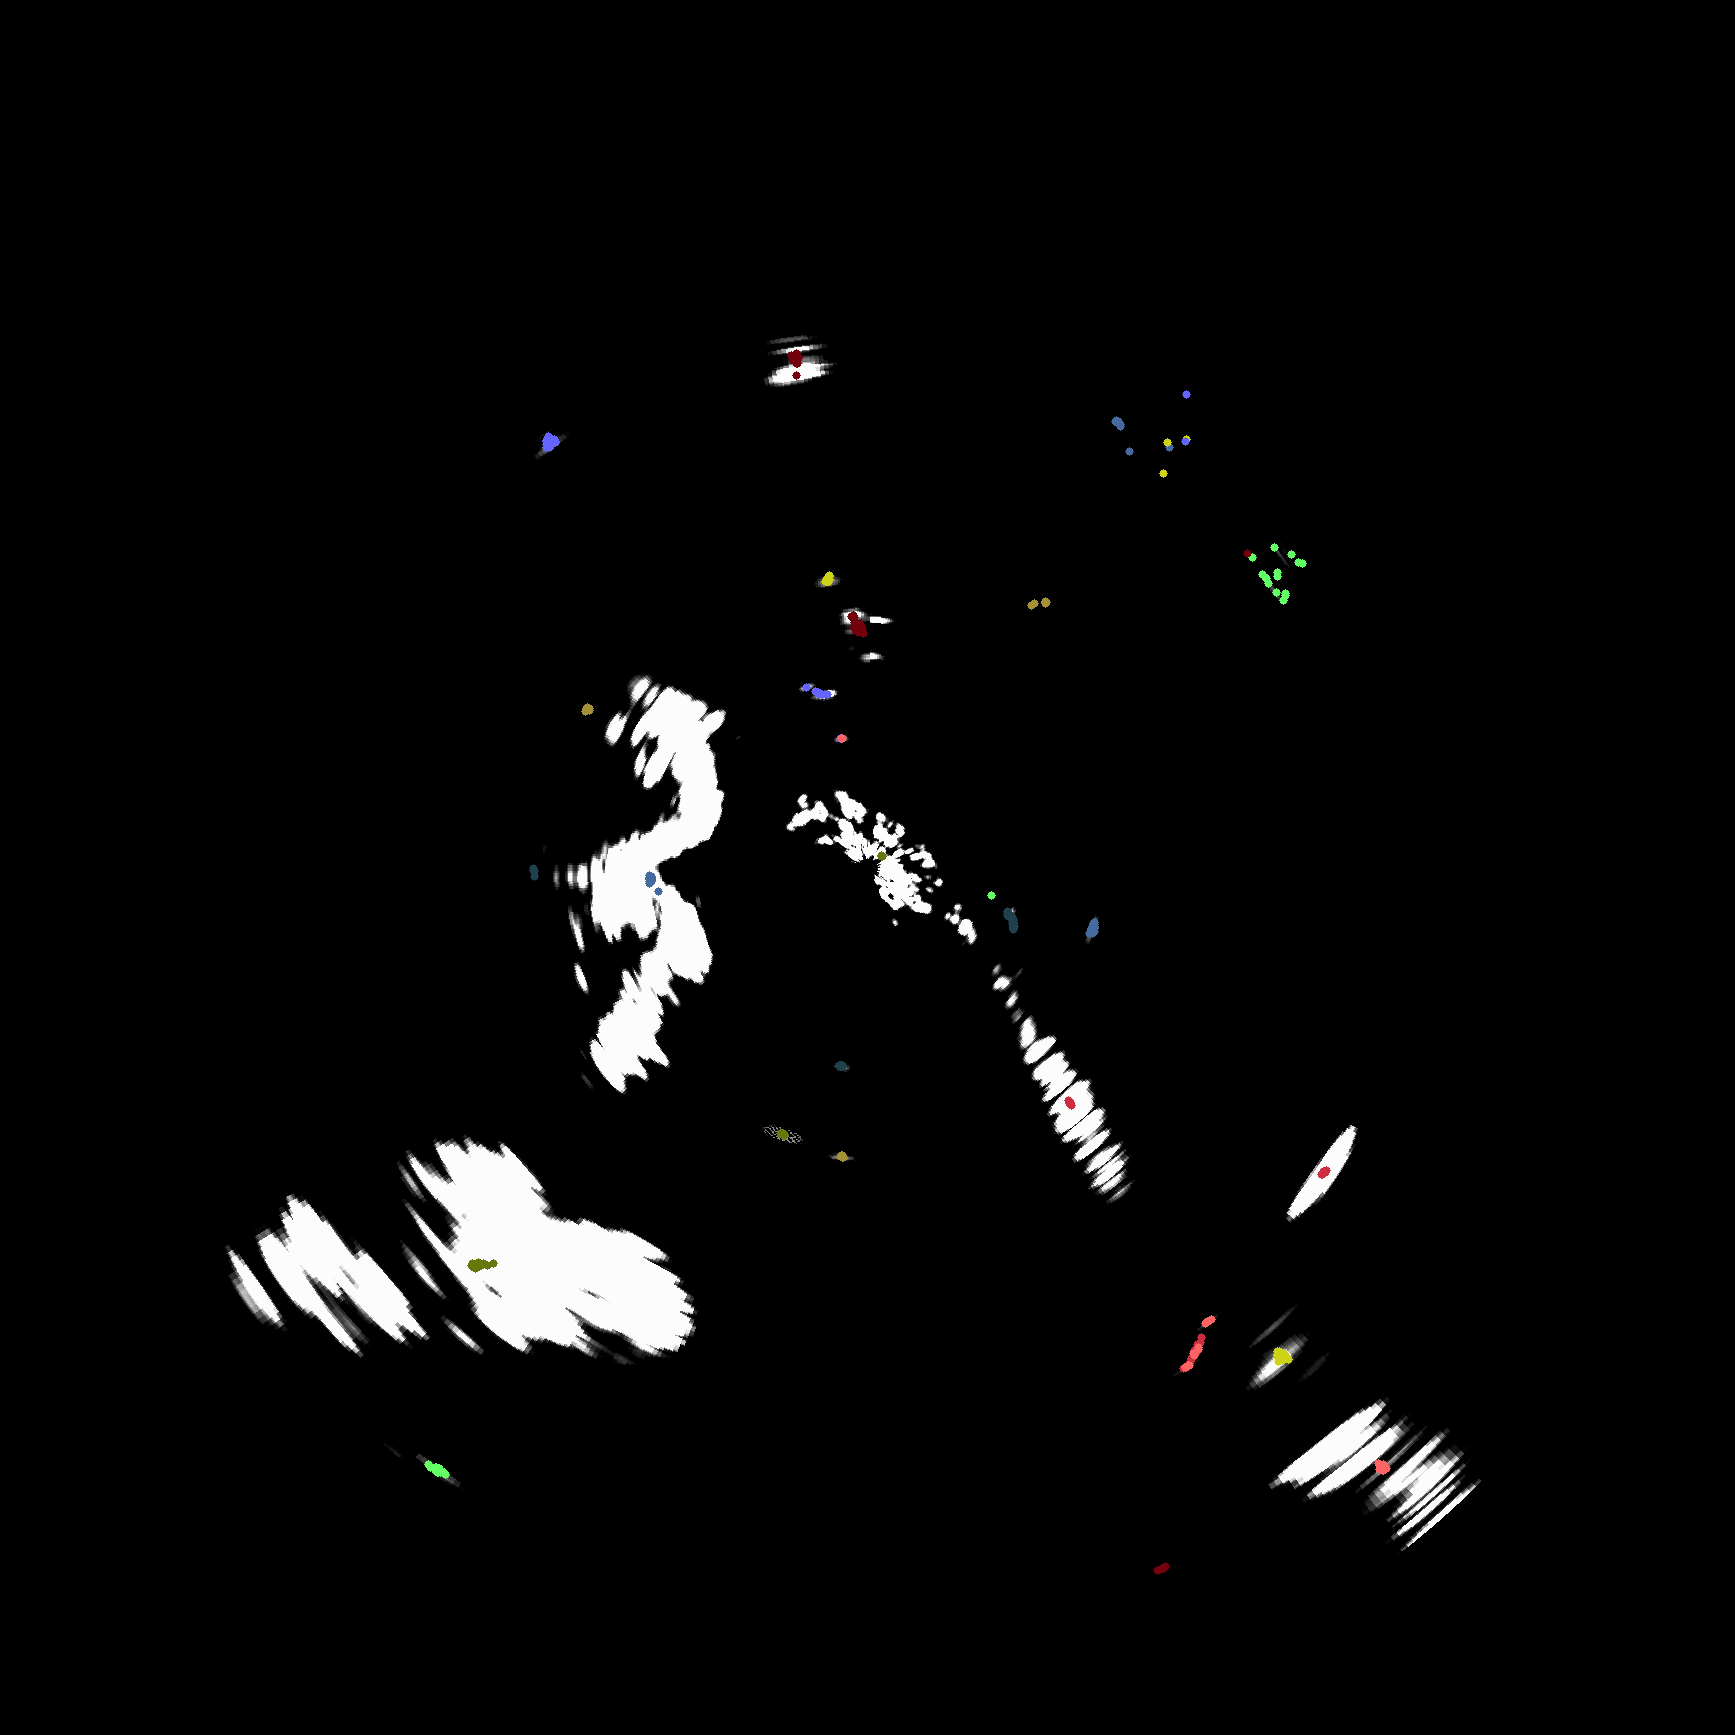
\includegraphics[width=0.31\textwidth]{figures/gap_track_frame.png}
\caption*{\scriptsize\textbf{Left:} Vanilla DBSCAN: 48 tracks, extensive false detections from land/clutter. \textbf{Center:} Adaptive ST-DBSCAN: 31 tracks, maintained target coverage. \textbf{Right:} Adaptive + Gap Recovery: 31 tracks, consolidated associations, zero ID switches.}
\end{figure}
\end{frame}

%=============================================================================
\begin{frame}{Results: MOT Metrics}
\scriptsize
\begin{columns}[T]
\column{0.58\textwidth}
\begin{table}
\centering
\tiny
\caption{Multi-Object Tracking Metrics on Synthetic Data}
\begin{tabular}{@{}lcccccc@{}}
\toprule
\textbf{Method} & \textbf{MOTA} & \textbf{MOTP} & \textbf{Recall} & \textbf{Prec.} & \textbf{FP} & \textbf{IDSW} \\
& & \textbf{(px)} & & & & \\
\midrule
Vanilla DBSCAN & $-6.97$ & 1.80 & 0.987 & 0.112 & 1208 & 18 \\
$\varepsilon_s=10$ & & & & & & \\[0.05cm]
Standard ST-DBSCAN & $-0.10$ & -- & 0.000 & 0.000 & 16 & 0 \\
$\varepsilon_s=10$, $\varepsilon_t=2$ & & & & & & \\[0.05cm]
Adaptive ST-DBSCAN & \textbf{$-4.44$} & \textbf{1.19} & \textbf{0.974} & 0.155 & 816 & 18 \\
$\varepsilon_{\min}=20$ & & & & & & \\[0.05cm]
\textcolor{Congaree}{\textbf{Adaptive + Gap}} & \textcolor{Congaree}{$-3.82$} & \textcolor{Congaree}{\textbf{1.18}} & \textcolor{Congaree}{0.812} & \textcolor{Congaree}{\textbf{0.159}} & \textcolor{Congaree}{\textbf{695}} & \textcolor{Congaree}{\textbf{0}} \\
\textcolor{Congaree}{$\tau=1$, $d=0.5$} & & & & & & \\
\bottomrule
\end{tabular}
\end{table}

\column{0.38\textwidth}
\textbf{Dataset:}
\begin{itemize}
  \setlength{\itemsep}{0pt}
  \item 50 frames
  \item 4 objects
  \item 15-40\% dropout rate
  \item 1735x1735 px
  \item 1847 signatures
\end{itemize}

\vspace{0.2cm}
\textbf{Key Findings:}
\begin{itemize}
  \setlength{\itemsep}{0pt}
  \item \textcolor{Rose}{Negative MOTA:} High-clutter environment
  \item \textcolor{Congaree}{Gap recovery eliminates ID switches}
  \item \textcolor{Congaree}{32\% FP reduction over vanilla DBSCAN}
  \item \textcolor{Congaree}{Best MOTP: 1.18 px localization}
\end{itemize}
\end{columns}
\end{frame}

%=============================================================================
\begin{frame}{Results: Per-Object Performance}
\begin{columns}[T]
\column{0.48\textwidth}
\begin{table}
\centering
\small
\caption{Per-Object Tracking (Vanilla DBSCAN)}
\begin{tabular}{@{}lccc@{}}
\toprule
\textbf{Object} & \textbf{Visible} & \textbf{Lifetime} & \textbf{MOTP (px)} \\
\midrule
Object 0 & 50 & 100\% & 1.01 \\
Object 1 & 50 & 100\% & 1.41 \\
Object 2 & 50 & 100\% & 1.16 \\
Object 3 & 4 & 50\% & 47.2 \\
\midrule
\textbf{Mean} & -- & 87.5\% & 12.7 \\
\bottomrule
\end{tabular}
\end{table}

\vspace{0.3cm}
\textbf{Observations:}
\begin{itemize}
  \scriptsize
  \item \textcolor{Congaree}{100\% lifetime} for persistent objects
  \item \textcolor{Congaree}{Sub-1.5 px MOTP} for tracked objects
  \item Object 3: brief appearance (4 frames)
  \item Initialization latency affects short tracks
\end{itemize}

\column{0.48\textwidth}
\begin{table}
\centering
\small
\caption{Timing Summary}
\begin{tabular}{@{}lc@{}}
\toprule
\textbf{Metric} & \textbf{Value} \\
\midrule
Total per sweep & 511 $\pm$ 93 ms \\
Throughput & \textasciitilde 2 sweeps/s \\
Real-time req. & 1.25 s/sweep \\
Memory usage & $<$ 500 MB \\
\midrule
\textbf{Margin} & \textbf{2.4$\times$} \\
\bottomrule
\end{tabular}
\end{table}

\vspace{0.3cm}
\textbf{Deployment Viability:}
\begin{itemize}
  \scriptsize
  \item Exceeds real-time by 2.4$\times$
  \item Headroom for latency spikes
  \item Low memory footprint
  \item Suitable for shipboard deployment
\end{itemize}
\end{columns}
\end{frame}

%=============================================================================
\begin{frame}{Limitations and Future Work}
\scriptsize
\begin{columns}[T]
\column{0.48\textwidth}
\textbf{Known Limitations:}
\begin{itemize}
  \setlength{\itemsep}{0pt}
  \item \textcolor{Rose}{Epsilon floor required} for dense data (less adaptive)
  \item \textcolor{Rose}{Synthetic evaluation only} (real radar pending)
  \item \textcolor{Rose}{Target crossing/merging} causes ID confusion
  \item \textcolor{Rose}{Stationary objects} hard to distinguish from clutter
  \item \textcolor{Rose}{Hyperparameters} ($k$, percentile) still manual
  \item \textcolor{Rose}{Dense point clouds} ($>$1M points) remain challenging
\end{itemize}

\vspace{0.15cm}
\textbf{Failure Cases:}
\begin{itemize}
  \setlength{\itemsep}{0pt}
  \item Multiple targets within $\varepsilon_s$ merge
  \item Extended path crossings cause persistent ID confusion
  \item Greedy Hungarian cannot disambiguate complex scenarios
\end{itemize}

\column{0.48\textwidth}
\textbf{Future Work:}
\begin{itemize}
  \setlength{\itemsep}{0pt}
  \item \textcolor{Congaree}{Kalman filtering} for velocity estimation
  \item \textcolor{Congaree}{Multi-hypothesis tracking} (MHT) for ambiguous associations
  \item \textcolor{Congaree}{AIS fusion} for supervised track identification
  \item \textcolor{Congaree}{3D extension} for vertically-scanning radars
  \item \textcolor{Congaree}{Geographic masking} to suppress land returns
  \item \textcolor{Congaree}{Real radar validation} with ground truth
  \item \textcolor{Congaree}{Adaptive temporal threshold} $\varepsilon_t$
\end{itemize}

\vspace{0.15cm}
\textbf{Application Domains:}
\begin{itemize}
  \setlength{\itemsep}{0pt}
  \item Autonomous maritime navigation
  \item Collision avoidance systems
  \item Harbor surveillance
  \item Search and rescue
\end{itemize}
\end{columns}
\end{frame}

%=============================================================================
{
\setbeamercolor{background canvas}{bg=Garnet}
\begin{frame}[plain,noframenumbering]
\vfill
\centering
{\Huge\textcolor{white}{\textbf{Questions?}}}\\[1.5cm]
{\large\textcolor{white}{S. Cancilla, J.C. Vaught, D. Cahl, Y. Wang}}\\[0.3cm]
{\large\textcolor{white}{University of South Carolina}}\\[0.2cm]
{\large\textcolor{white}{Columbia, SC 29208}}\\[1.5cm]
{\normalsize\textcolor{white}{AIAA Region II Student Conference 2026}}
\vfill
\end{frame}
}

\end{document}
